\documentclass{article}
\usepackage{graphicx} % Required for inserting images
\usepackage[a4paper,margin=1in]{geometry}
\usepackage{amsmath}
\usepackage{amssymb}
\usepackage{graphicx}
\usepackage{booktabs}
\usepackage{hyperref}


\usepackage{float}
\usepackage{tikz}
\usepackage{pgfplots}
\pgfplotsset{compat=1.18}

\usepackage{float}

\begin{document}
\begin{titlepage}
\centering

\vspace*{2cm}

{\Huge\bfseries
Currency + Commodity Risk Joint Hedging:
Optimal Hedging of African Commodity Exposure Under FX Risk
\par}

\vspace{1.5cm}

{\Large Great Hanson}

\vspace{0.5cm}

Department of Business and Information Technology\\
Ontario Tech University

\vfill

Research Paper

\vspace{0.5cm}

\today

\vfill

Copyright \textcopyright\ 2026 Great Hanson

\end{titlepage}

\begin{abstract}
Commodity exporting African economies are highly vulnerable to external shocks arising from fluctuations in both global commodity prices and foreign exchange markets. Because commodities such as crude oil, cocoa, gold, and copper account for a substantial share of export revenues and government income, movements in commodity markets frequently transmit into exchange-rate volatility, inflationary pressures, and broader macroeconomic instability. Traditional risk management frameworks generally hedge commodity price risk and currency risk separately, despite evidence that these exposures are closely interconnected in resource dependent emerging markets.

This study investigates whether a joint hedging framework that simultaneously incorporates commodity and foreign exchange risk can improve risk adjusted outcomes relative to isolated hedging strategies. Using historical data from major African commodity exporting economies, including Nigeria, Ghana, South Africa, Congo, Algeria, and Zambia, the analysis examines the dynamic relationships between commodity prices, exchange rates, and export dependence across different macroeconomic environments. The research employs rolling correlation analysis, rolling beta estimation, volatility transmission models, and minimum variance hedge ratio techniques to evaluate how commodity currency linkages evolve over time. Particular attention is given to the effects of global inflation cycles, U.S. dollar strength, monetary tightening, commodity super cycles, and recessionary regimes on hedging effectiveness.

The findings suggest that the magnitude and direction of foreign-exchange sensitivity to commodity markets vary significantly across countries and time periods, indicating that static hedging approaches may be insufficient for managing export-related risks. Consequently, the paper argues that integrated hedging strategies that jointly account for commodity and currency exposures provide a more effective framework for risk mitigation in African commodity dependent economies. By identifying the conditions under which joint hedging delivers superior performance, this research contributes to the growing literature on integrated risk management and offers practical implications for policymakers, sovereign wealth funds, multinational corporations, and institutional investors seeking to improve resilience against global market shocks while preserving export revenue stability.

\vspace{0.5em}
\noindent
\textbf{Keywords:} Commodity Risk, Foreign Exchange Risk, Joint Hedging, African Commodity Exporters, Minimum-Variance Hedging, Exchange Rate Exposure, Commodity Supercycles, Portfolio Risk Management.

\end{abstract}

\newpage
\tableofcontents
\newpage
\begin{center}
{\Large \textbf{ Introduction}}
\end{center}
Commodity markets and foreign exchange markets are among the most important drivers of economic performance in many African economies. Across the continent, exports of crude oil, gold, cocoa, copper, natural gas, agricultural products, and industrial metals generate substantial foreign exchange earnings and government revenues. Consequently, fluctuations in global commodity prices often influence not only trade balances and economic growth but also exchange-rate stability, inflation dynamics, and broader financial conditions.

Despite the economic importance of commodities, African currencies have exhibited dramatically different performance over the past decade. While some currencies have remained relatively stable against the U.S. dollar, others have experienced substantial periods of depreciation and volatility. These differences raise an important question: to what extent are exchange-rate movements driven by underlying commodity exposures, and how stable are these relationships through time?

Conventional wisdom suggests that commodity-exporting countries should benefit from rising commodity prices and suffer during commodity downturns. However, real-world outcomes are often more complex. Periods of rising oil prices do not always coincide with stronger oil-exporting currencies, while commodity booms can occur alongside persistent currency weakness. Global inflation shocks, shifts in U.S. monetary policy, changes in Chinese demand, and domestic macroeconomic conditions may alter or even overwhelm commodity-driven effects. As a result, the relationship between commodities and exchange rates is likely to be dynamic rather than constant.

Understanding these dynamics is particularly important from a risk-management perspective. Commodity producers, exporters, governments, and investors are frequently exposed to both commodity price risk and foreign exchange risk simultaneously. Yet these risks are often analyzed and hedged independently. Such an approach may overlook important interactions between commodity markets and currency movements, potentially reducing the effectiveness of traditional hedging strategies.

This study investigates the relationship between major commodity markets and African currencies using a cross-country framework that combines commodity price data, exchange-rate data, and country-level measures of export dependence. The analysis includes energy commodities, precious metals, industrial metals, and agricultural commodities alongside a broad sample of African exchange rates. By examining currency devaluation patterns, commodity betas, rolling correlations, volatility transmission mechanisms, and macroeconomic regimes, the paper seeks to identify which currencies exhibit the strongest commodity characteristics and how these relationships evolve over time.

Building upon this foundation, the study evaluates whether joint commodity and foreign exchange hedging strategies can improve risk management outcomes relative to commodity-only or currency-only approaches. Particular attention is given to the role of macroeconomic regimes, including inflation shocks, Federal Reserve tightening cycles, commodity supercycles, and periods of global economic stress.

The contribution of this paper is threefold. First, it provides a comprehensive analysis of commodity--currency linkages across a diverse sample of African economies. Second, it examines the extent to which these relationships change through time and across different economic environments. Third, it applies these findings within a practical hedging framework to assess whether integrated management of commodity and foreign exchange exposures can provide superior protection against external shocks.

The paper is guided by the following research questions:

\begin{enumerate}
    \item Which African currencies have experienced the greatest degree of devaluation against the U.S. dollar over the past five years?
    
    \item Which African currencies exhibit the strongest characteristics of commodity currencies?
    
    \item To what extent do commodity price movements transmit into exchange-rate dynamics?
    
    \item How do commodity--currency relationships evolve across different macroeconomic regimes?
    
    \item Do dynamic commodity--FX relationships imply that hedge ratios should also be dynamic?
    
    \item Does jointly hedging commodity and foreign exchange exposure provide superior risk-adjusted outcomes relative to isolated hedging approaches?
\end{enumerate}

The remainder of the paper proceeds as follows. Section 2 reviews the relevant literature on commodity risk, foreign exchange risk, and hedging strategies. Section 3 examines currency devaluation and commodity dependence across African economies. Sections 4 through 6 analyze commodity--currency relationships using correlation analysis, rolling correlations, volatility transmission measures, and commodity beta models. Sections 7 through 9 develop and evaluate hedging strategies under different macroeconomic regimes. The final sections discuss the empirical findings, policy implications, and conclusions.

\newpage
\section{Literature Review}

\subsection{Commodity Risk in Emerging Markets}

Commodity risk refers to the uncertainty associated with fluctuations in the prices of raw materials and primary commodities. For many emerging-market economies, commodity exports represent a major source of foreign exchange earnings, government revenue, and economic growth. Consequently, changes in commodity prices can have significant implications for economic stability, fiscal performance, and financial markets.

Commodity-dependent economies are particularly vulnerable to external shocks because their export structures are often concentrated in a small number of products. Declines in commodity prices can reduce export revenues, weaken trade balances, and increase macroeconomic instability. Previous research has shown that commodity price volatility is frequently associated with exchange-rate fluctuations, inflationary pressures, and economic downturns in resource-dependent economies.

The importance of commodity risk is particularly evident in Africa, where many economies rely heavily on exports of crude oil, copper, gold, cocoa, and other primary commodities. As a result, understanding the transmission of commodity shocks into financial markets remains an important area of research for both policymakers and investors.

\subsection{Foreign Exchange Risk and Currency Devaluation}

Foreign exchange risk refers to the potential for losses arising from changes in exchange rates. In emerging markets, exchange-rate movements are influenced by a combination of domestic economic conditions and external factors, including commodity prices, capital flows, monetary policy, and global financial conditions.

Currency devaluation can have substantial economic consequences. Depreciation increases the local currency cost of imports, contributes to inflationary pressures, and may reduce investor confidence. Over the past decade, several African currencies have experienced significant depreciation against the U.S. dollar, reflecting varying degrees of macroeconomic vulnerability and exposure to external shocks.

Recent evidence from African economies highlights considerable differences in currency performance. While the Nigerian naira and Ethiopian birr experienced substantial depreciation, other currencies such as the Algerian dinar and South African rand exhibited greater relative stability. These differences suggest that exchange-rate dynamics cannot be explained by commodity exposure alone and may reflect broader economic and institutional factors.

\subsection{Commodity Currencies and Terms-of-Trade Effects}

The concept of a commodity currency refers to a currency whose value is strongly influenced by changes in the prices of commodities exported by the underlying economy. The theoretical foundation for commodity currencies is rooted in the terms-of-trade framework, which suggests that improvements in export prices increase national income, strengthen external balances, and support currency appreciation.

Countries heavily dependent on commodity exports are generally expected to exhibit stronger relationships between commodity prices and exchange rates. For example, increases in oil prices may improve export revenues for oil-exporting countries, while rising copper prices may strengthen economies dependent on copper production. Conversely, commodity price declines can reduce foreign exchange inflows and place downward pressure on domestic currencies.

Previous studies have documented commodity-currency relationships in both developed and emerging economies. However, the strength and stability of these relationships vary significantly across countries and time periods. This variation suggests that commodity-currency linkages may be dynamic rather than constant, particularly in emerging-market economies subject to changing macroeconomic conditions.

\subsection{Joint Hedging Frameworks}

Traditional risk-management frameworks often treat commodity price risk and foreign exchange risk as separate sources of uncertainty. Commodity producers commonly hedge output prices through futures contracts, while currency exposures are managed independently through foreign exchange derivatives.

Recent research suggests that such an approach may be insufficient for commodity-exporting economies. Commodity price declines can simultaneously reduce export revenues and weaken domestic currencies, creating multiple channels through which losses occur. Consequently, managing commodity and foreign exchange risk independently may fail to capture important interactions between these risk factors.

Joint hedging frameworks seek to address this limitation by integrating commodity and currency exposures within a unified risk-management strategy. By accounting for the interaction between commodity markets and exchange rates, joint hedging approaches may provide superior risk-adjusted outcomes relative to isolated hedging methods.

\subsection{Dynamic Hedge Ratios}

The effectiveness of a hedging strategy depends on the hedge ratio, which determines the proportion of exposure offset through derivative positions. Traditional hedging approaches frequently employ static hedge ratios estimated using historical data.

However, financial relationships often evolve through time. Correlations between assets may strengthen during periods of market stress and weaken during more stable conditions. Consequently, static hedge ratios may become ineffective when market dynamics change.

To address this issue, researchers have developed dynamic hedging approaches that allow hedge ratios to vary over time. Methods such as rolling-window estimation, time-varying regression models, and multivariate volatility models have been widely employed to capture changing market relationships. Dynamic hedging frameworks are particularly relevant when commodity-currency relationships exhibit substantial variation across economic regimes.

Evidence from African commodity-exporting economies suggests that commodity sensitivities and correlations fluctuate considerably through time. Such findings provide a strong rationale for evaluating dynamic hedging strategies alongside traditional static approaches.

\subsection{African Commodity Export Economies}

African economies provide a particularly relevant setting for examining the interaction between commodity prices and exchange rates. Many countries remain heavily dependent on commodity exports for foreign exchange earnings, fiscal revenues, and economic growth. However, the degree of commodity dependence varies substantially across economies.

Among the countries examined in this study, Algeria and Nigeria exhibit the highest levels of export concentration, with mineral fuels accounting for approximately 91.5\% and 83.6\% of total exports, respectively. The Democratic Republic of the Congo and Zambia are heavily dependent on copper exports, which account for approximately 70.6\% and 67.3\% of export revenues. Ghana derives approximately 67.9\% of export earnings from gold and cocoa exports, while South Africa maintains a comparatively diversified export structure, with precious metals accounting for approximately 20.3\% of exports.

These differences in export concentration suggest that commodity price shocks may affect exchange rates differently across countries. Highly concentrated exporters may exhibit stronger commodity-currency relationships due to their greater dependence on a single source of foreign exchange earnings. More diversified economies, however, may be less sensitive to fluctuations in individual commodity markets.

Despite a substantial literature on commodity risk, foreign exchange risk, and hedging strategies, relatively limited attention has been devoted to the joint management of commodity and currency exposures within African economies. Furthermore, existing studies rarely examine how commodity-currency relationships evolve across different macroeconomic regimes. This study seeks to address these gaps by integrating commodity prices, exchange rates, export dependence, and dynamic hedging strategies within a unified framework focused on African commodity-exporting economies.

\subsection{Commodity Risk in Emerging Markets}

Commodity price volatility represents one of the most significant sources of economic uncertainty in emerging markets. Unlike diversified developed economies, many emerging-market countries rely heavily on a narrow range of primary commodities for export earnings, government revenue, and foreign exchange inflows. Consequently, fluctuations in global commodity prices can have widespread implications for economic growth, fiscal stability, and financial market performance.

The transmission of commodity shocks is particularly pronounced in resource-dependent economies. Rising commodity prices generally improve trade balances and increase export revenues, while declining prices can weaken external accounts and contribute to economic instability. Previous research has shown that commodity price cycles frequently coincide with periods of elevated exchange-rate volatility and macroeconomic stress in emerging markets.

The African economies examined in this study are particularly exposed to commodity risk due to their reliance on exports of crude oil, copper, gold, cocoa, and other primary commodities. As a result, understanding the interaction between commodity markets and financial variables remains an important area of research.

\subsection{Foreign Exchange Risk and Currency Devaluation}

Foreign exchange risk refers to the uncertainty arising from fluctuations in exchange rates. For commodity-exporting economies, exchange-rate movements influence trade competitiveness, inflation, capital flows, and the value of foreign-denominated liabilities. As a result, currency instability can create substantial economic and financial risks.

Over the past decade, several African currencies have experienced significant depreciation against the U.S. dollar. Currency weakness may result from a variety of factors, including inflationary pressures, deteriorating trade balances, external debt burdens, monetary policy decisions, and adverse commodity-price shocks. In highly commodity-dependent economies, reductions in export earnings can place downward pressure on domestic currencies by reducing foreign exchange inflows.

The substantial variation in exchange-rate performance across African economies suggests that currency movements are influenced by both commodity-related and macroeconomic factors. Consequently, understanding the determinants of currency devaluation remains essential for evaluating financial vulnerability and risk-management strategies.

\subsection{Commodity Currencies and Terms-of-Trade Effects}

The concept of a commodity currency refers to a currency whose value is significantly influenced by the prices of commodities exported by the underlying economy. Commodity-currency relationships are commonly explained through terms-of-trade effects, which describe how changes in export prices influence national income, trade balances, and exchange rates.

When commodity prices increase, export revenues rise, often leading to stronger external balances and increased demand for domestic currency. Conversely, commodity price declines may reduce export earnings and weaken exchange-rate performance. Previous studies have documented such relationships in both developed and emerging-market economies.

However, commodity-currency relationships are rarely constant through time. Changes in global economic conditions, monetary policy, investor sentiment, and domestic economic fundamentals may alter the strength and direction of commodity-currency linkages. This study investigates whether African currencies exhibit characteristics consistent with commodity currencies and whether these relationships remain stable across different market environments.

\subsection{Joint Hedging Frameworks}

Traditional risk-management approaches typically treat commodity price risk and foreign exchange risk as separate sources of uncertainty. Commodity producers frequently hedge output prices through futures contracts, while currency exposures are managed independently through foreign exchange derivatives.

Such an approach may be insufficient for commodity-exporting economies because commodity and currency risks are often interconnected. A decline in commodity prices can simultaneously reduce export revenues and weaken the domestic currency, exposing economic agents to multiple sources of loss. Consequently, separate hedging strategies may fail to capture important interactions between commodity markets and exchange-rate movements.

Joint hedging frameworks seek to address this limitation by incorporating commodity and foreign exchange exposures within a unified risk-management strategy. By recognizing the interconnected nature of these risks, integrated hedging approaches may provide greater protection against external shocks and improve overall hedging effectiveness.

\subsection{Dynamic Hedge Ratios}

The effectiveness of any hedging strategy depends critically on the hedge ratio, which determines the proportion of exposure offset through derivative positions. Traditional approaches often rely on static hedge ratios estimated from historical relationships between assets.

However, financial markets are inherently dynamic. Correlations between commodities and exchange rates frequently change over time in response to economic conditions, policy decisions, and periods of financial stress. As a result, static hedge ratios may become less effective when market relationships evolve.

To address this issue, researchers have developed dynamic hedging frameworks that allow hedge ratios to adjust through time. Methods such as rolling-window estimation and time-varying volatility models have become increasingly common in the risk-management literature. The evidence presented later in this study suggests that commodity-currency relationships vary considerably across time and economic regimes, providing strong motivation for evaluating dynamic hedging strategies alongside traditional static approaches.

\subsection{African Commodity Export Economies}

African economies provide a particularly relevant setting for examining the interaction between commodity prices and exchange rates. Many countries remain highly dependent on commodity exports for foreign exchange earnings, fiscal revenues, and economic growth. However, the degree of commodity dependence varies substantially across economies.

Among the countries examined in this study, Algeria and Nigeria exhibit the highest levels of export concentration, with mineral fuels accounting for approximately 91.5\% and 83.6\% of total exports, respectively. The Democratic Republic of the Congo and Zambia rely heavily on copper exports, which account for approximately 70.6\% and 67.3\% of export revenues. Ghana derives approximately 67.9\% of export earnings from gold and cocoa exports, while South Africa maintains a comparatively diversified export structure, with precious metals accounting for approximately 20.3\% of exports.

\begin{figure}[H]
\centering

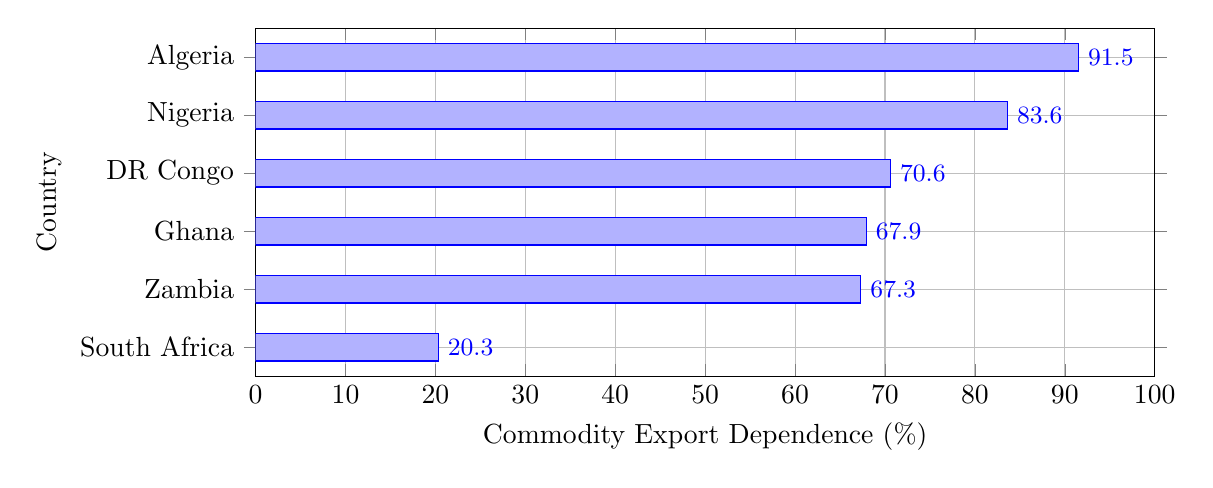
\begin{tikzpicture}
\begin{axis}[
xbar,
width=13cm,
height=6cm,
xlabel={Commodity Export Dependence (\%)},
ylabel={Country},
xmin=0,
xmax=100,
ytick=data,
yticklabels={
South Africa,
Zambia,
Ghana,
DR Congo,
Nigeria,
Algeria
},
nodes near coords,
every node near coord/.append style={font=\small},
grid=major
]

\addplot coordinates {
(20.3,0)
(67.3,1)
(67.9,2)
(70.6,3)
(83.6,4)
(91.5,5)
};

\end{axis}
\end{tikzpicture}
\caption{Commodity Export Dependence by Country}
\label{fig:export_dependence}
\end{figure}


Figure \ref{fig:export_dependence} highlights the substantial variation in commodity dependence across the sample economies. Algeria and Nigeria derive the overwhelming majority of their export earnings from energy products, while Zambia and the Democratic Republic of the Congo remain heavily dependent on copper exports. Ghana relies primarily on gold and cocoa exports, whereas South Africa exhibits a comparatively diversified export structure.

These differences in export concentration suggest that commodity price shocks may affect exchange rates differently across countries. Highly concentrated exporters are expected to exhibit stronger commodity--currency relationships because fluctuations in commodity prices directly affect foreign exchange inflows and trade balances. More diversified economies may be less sensitive to shocks affecting individual commodity markets.

Despite a substantial literature on commodity risk, foreign exchange risk, and hedging strategies, relatively limited attention has been devoted to the joint management of commodity and currency exposures within African economies. Furthermore, existing studies rarely examine how commodity--currency relationships evolve across different macroeconomic regimes. This study seeks to address these gaps by integrating commodity prices, exchange rates, export dependence, and dynamic hedging strategies within a unified framework focused on African commodity-exporting economies.

\section{African Currency Devaluation: A Macro Perspective}

Exchange-rate performance is a critical indicator of macroeconomic stability in emerging and developing economies. Currency movements influence inflation, trade competitiveness, external debt servicing costs, and the value of foreign-denominated assets and liabilities. For commodity-exporting economies, exchange-rate fluctuations are particularly important because export earnings are frequently concentrated in a limited number of globally traded commodities.

Over the past decade, African currencies have experienced varying degrees of depreciation against the U.S. dollar. While some currencies have undergone substantial devaluations, others have remained comparatively stable despite exposure to similar external shocks. These differences raise important questions regarding the role of commodity dependence, inflation, sovereign risk, and macroeconomic policy in shaping exchange-rate outcomes.

The objective of this chapter is to examine patterns of currency devaluation across the six African economies included in this study and identify potential factors that may explain observed differences in exchange-rate performance. The analysis provides a macroeconomic foundation for the commodity--currency relationships explored in subsequent chapters.

\subsection{Five-Year Currency Devaluation Ranking}

To evaluate exchange-rate performance, the percentage change in each currency relative to the U.S. dollar was calculated using:

\[
\%\Delta FX =
\left(
\frac{FX_{Final}}
{FX_{Initial}}
-1
\right)
\times100
\]

where $FX_{Initial}$ and $FX_{Final}$ represent the beginning and ending exchange rates over the sample period.

The results indicate substantial variation in currency performance across African economies. The Ethiopian birr, Nigerian naira, and Egyptian pound experienced the largest depreciations against the U.S. dollar, while the Algerian dinar remained comparatively stable. The Zambian kwacha was the only currency in the sample to record an overall appreciation during the period.

\begin{figure}[H]
\centering

\includegraphics[width=0.9\textwidth]{fx_devaluation_5y.png}
\caption{Five-Year Currency Devaluation Ranking}
\label{fig:devaluation_ranking}
\end{figure}

The magnitude of these differences highlights the heterogeneous nature of exchange-rate dynamics across African economies and suggests that multiple economic factors contribute to currency performance.

\subsection{Normalized Commodity and Currency Performance}

While the devaluation ranking summarizes cumulative currency performance, it does not capture the timing and evolution of exchange-rate movements. To address this limitation, normalized indices were constructed by setting all commodities and exchange rates equal to 100 at the beginning of the sample period.

\begin{figure}[H]
\centering
\includegraphics[width=0.95\textwidth]{normalized_macro_factor_map_5y.png}
\caption{Normalized Commodity and Foreign Exchange Performance (Base = 100)}
\label{fig:normalized_fx}
\end{figure}

The normalized performance indices provide a comparative view of commodity prices and exchange rates over the sample period. By setting all series equal to 100 at the beginning of the sample, differences in relative performance become easier to observe.

Several important patterns emerge. First, substantial divergence exists among the currencies included in the analysis. The Nigerian naira and Ghanaian cedi experienced pronounced depreciation relative to the U.S. dollar, while the Zambian kwacha displayed considerably greater stability. Second, commodity prices exhibited significant cyclical fluctuations throughout the sample period. Cocoa recorded the strongest overall performance, while copper and crude oil experienced periods of both expansion and contraction.

The figure also suggests that commodity and currency movements do not always occur simultaneously. While certain periods appear characterized by co-movement between commodities and exchange rates, other periods exhibit substantial divergence. These observations provide preliminary evidence that commodity--currency relationships may vary through time and motivate the rolling correlation and commodity beta analyses conducted in later chapters.

\subsection{Inflation and Currency Instability}

Inflation is widely recognized as an important determinant of exchange-rate performance. Persistent inflation reduces purchasing power and may weaken investor confidence, placing downward pressure on domestic currencies.

For commodity-exporting economies, inflationary pressures may arise from a combination of domestic and external factors, including food and energy prices, fiscal deficits, exchange-rate pass-through effects, and monetary expansion. Elevated inflation often coincides with periods of exchange-rate volatility, creating feedback mechanisms that reinforce macroeconomic instability.

Although inflation is not the sole determinant of currency performance, it remains an important channel through which economic shocks influence exchange rates in emerging markets.

\subsection{Sovereign Risk and Exchange Rate Credibility}

Exchange-rate outcomes are also influenced by sovereign risk and the credibility of economic institutions. Countries with stronger fiscal positions, larger foreign exchange reserves, and more credible monetary policy frameworks are often better positioned to withstand external shocks.

The comparison between Algeria and Nigeria illustrates this point. Both economies are highly dependent on energy exports, yet their currencies exhibited substantially different performance during the sample period. Such differences suggest that commodity dependence alone is insufficient to explain exchange-rate dynamics.

Political stability, reserve management, debt sustainability, and central bank credibility may all influence a country's ability to maintain exchange-rate stability during periods of external stress.

\subsection{Commodity Dependence and Currency Weakness}

Commodity dependence represents a potential mechanism through which commodity-price fluctuations influence exchange-rate performance. Economies that derive a large proportion of export earnings from a single commodity may be more vulnerable to external shocks because changes in commodity prices directly affect foreign exchange inflows.

Table \ref{tab:export_dependence} summarizes the commodity export dependence of the six economies examined in this study.

\begin{table}[H]
\centering
\caption{Commodity Export Dependence by Country}
\label{tab:export_dependence}
\begin{tabular}{lcc}
\hline
Country & Primary Commodity & Export Share (%) \\
Algeria & Oil and Natural Gas & 91.5 \\
Nigeria & Oil & 83.6 \\
DR Congo & Copper & 70.6 \\
Ghana & Gold and Cocoa & 67.9 \\
Zambia & Copper & 67.3 \\
South Africa & Precious Metals & 20.3 \\
\hline
\end{tabular}
\end{table}


\vspace{0.2cm}


{\footnotesize
\textit{Note: Export dependence is measured as the percentage of total exports attributable to the country's primary commodity export category.}
}



The figure highlights substantial differences in export concentration. Algeria and Nigeria derive the overwhelming majority of export earnings from energy products, while Zambia and the Democratic Republic of the Congo remain heavily dependent on copper exports. Ghana relies primarily on gold and cocoa exports, whereas South Africa maintains a more diversified export structure.

These differences suggest that commodity-price shocks may influence exchange rates differently across countries and provide a potential explanation for variation in currency performance.

\subsection{Stylized Facts and Preliminary Observations}

Several stylized facts emerge from the preceding analysis.

First, significant differences exist in exchange-rate performance across African economies. Second, countries with high levels of commodity dependence do not necessarily exhibit similar currency outcomes. Third, commodity concentration alone appears insufficient to explain exchange-rate dynamics, suggesting that broader macroeconomic factors play an important role.

These findings motivate a more detailed investigation of commodity--currency relationships in subsequent chapters. In particular, the observed variation across countries raises important questions regarding whether African currencies behave as commodity currencies and whether these relationships remain stable through time. The next chapter addresses these questions through an examination of commodity-price dynamics, exchange-rate behavior, and commodity-currency linkages.


\section{Market System Analysis}

\subsection{Commodity Price Dynamics}

\subsection{Exchange Rate Dynamics}

\subsection{Normalized Asset Performance}

\subsection{Commodity–FX Correlation Matrix}

\subsection{Rolling Correlation Analysis}

\subsection{Volatility Transmission}

\subsection{Inflation Linkages}

\section{Commodity Currency Characteristics}

\subsection{Commodity Beta Methodology}

\subsection{Oil Beta: Nigeria}

\subsection{Gold and Cocoa Beta: Ghana}

\subsection{Copper Beta: Zambia}

\subsection{Gold and Precious Metals Beta: South Africa}

\subsection{Commodity Currency Ranking}

\subsection{Which Currencies Behave Most Like Commodity Currencies?}

\section{Fundamental Overlay}

\subsection{Export Dependency Ratios}

\subsection{Commodity Production Profiles}

\subsection{Export Revenue Concentration}

\subsection{Country Weighting Framework}

\subsection{Commodity Dependence Score}

\section{Optimal Hedging Framework}

\subsection{Minimum Variance Hedging}

\subsection{Static Hedge Ratios}

\subsection{Dynamic Hedge Ratios}

\subsection{Rolling Hedge Effectiveness}

\subsection{Commodity-Only Hedging}

\subsection{FX-Only Hedging}

\subsection{Joint Commodity and FX Hedging}

\subsection{Comparative Hedging Performance}

\section{Macroeconomic Regime Analysis}

\subsection{Federal Reserve Tightening Cycles}

\subsection{Global Inflation Shock Regimes}

\subsection{Commodity Supercycles}

\subsection{China Demand Shocks}

\subsection{Global Recession Regimes}

\subsection{Regime-Dependent Commodity Betas}

\subsection{Regime-Dependent Hedge Ratios}

\section{Stress Testing and Risk Analysis}

\subsection{Historical Crisis Analysis}

\subsection{Commodity Price Collapse Scenarios}

\subsection{USD Appreciation Scenarios}

\subsection{Inflation Shock Scenarios}

\subsection{Tail-Risk Analysis}

\subsection{Hedging Performance Under Stress}

\section{Empirical Results and Discussion}

\subsection{Does Commodity Regime Transmit into FX?}

\subsection{Are African Exporters Leveraged Bets on Global Inflation?}

\subsection{Which Countries Are Most Sensitive to Global Downturns?}

\subsection{Do Dynamic Hedges Outperform Static Hedges?}

\subsection{Does Joint Hedging Deliver Superior Risk-Adjusted Outcomes?}

\section{Policy Implications}

\subsection{Central Bank Reserve Management}

\subsection{Sovereign Wealth Funds}

\subsection{Commodity Exporters}

\subsection{Institutional Investors}

\section{Conclusion}

\newpage

\appendix

\section{Data Sources and Construction}

\section{Currency Devaluation Calculations}

\section{Correlation and Rolling Correlation Models}

\section{Commodity Beta Regression Models}

\section{Minimum Variance Hedge Derivations}

\section{Dynamic Hedge Ratio Models}

\section{Additional Tables}

\section{Additional Figures}

\section{Robustness Tests}

\newpage



\bibliographystyle{plain}
\bibliography{references}
\end{document}
